\documentclass[a4paper,10pt]{leaflet}

% French language
\usepackage[francais]{babel}
\usepackage[utf8]{inputenc}

% Hack
\setlength{\footskip}{10cm}

% No indentation but a wider space between the paragraphs
\setlength{\parindent}{0cm}
\setlength{\parskip}{2mm}

% To include images
\usepackage{graphicx}

\usepackage{multicol}

% Math extensions
\usepackage{amsfonts}
\usepackage{amstext}
\usepackage{amsmath}
\usepackage{mathbbol}

% Some useful shortcuts
\newcommand{\code}[1]{\mathcal{#1}}
\newcommand{\C}{\code{C}}
\newcommand{\syn}[1]{\mathop{\rm{syn}}(#1)}
\newcommand{\dimc}[1]{\mathop{\rm{dim}}(#1)}
\newcommand{\FF}{\mathbb{F}_2}
\newcommand{\FFn}[1]{\mathbb{F}_2^{#1}}


\title{Codes correcteurs \\ {\normalsize \textsf{Cheat Sheet}}}
\author{Nicolas MASSE \\ \texttt{nicolas27.masse@laposte.net}}

\begin{document}
\maketitle

\fussy

\section{Système de communication}
\subsection{Modèle de Shannon (1948)}
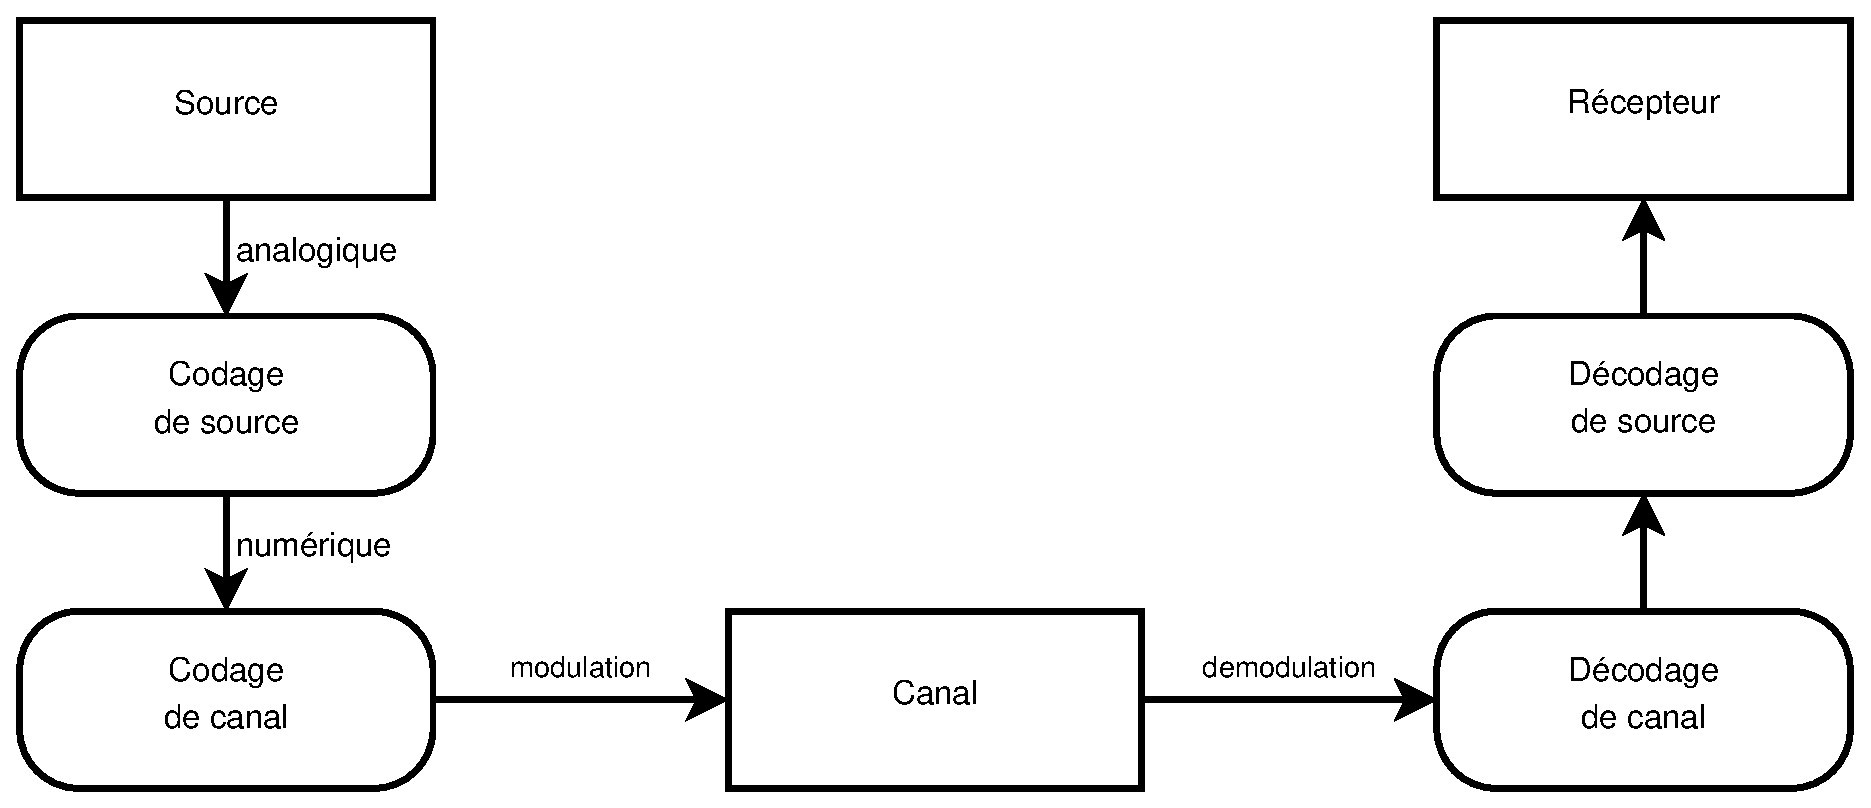
\includegraphics[width=0.9\linewidth]{general2}

\subsection{Matrice stochastique}
Une matrice stochastique $\mathcal{P}$ est définie par $ \mathcal{P} = (P_{ij}) $. $P_{ij} = P(y_j/x_i)$ est la probabilité de transition entre $x_i$ et $y_j$.

\subsection{Modèles de canal}

\begin{multicols}{2}
 \raggedcolumns
 Le \textbf{canal binaire symétrique à effacement} modélise les situations où certains symboles sont perdus.

\begin{center}
 $ \mathcal{P} = \begin{pmatrix}
 1-p & 0 & p\\
 0 & 1-p & p\\
 \end{pmatrix}$
\end{center}

 \includegraphics[width=0.9\linewidth]{cbse}
\end{multicols}
\clearpage
\begin{multicols}{2}
 \raggedcolumns
 \textbf{Canal binaire symétrique}

\begin{center}
$ \mathcal{P} = \left(
\begin{array}{cc}
 1-p & p\\
 p & 1-p\\
\end{array}
\right)$
\end{center}

 \includegraphics[width=\linewidth]{cbs}
\end{multicols}

\subsection{Codage de source}
Une source est équiprobable lorsque chaque séquence binaire a la même probabilité d'apparition.
On dit alors que le codage de source est de qualité.

\section{Théorie des codes}

\subsection{Types de codes}
\begin{itemize}
 \item codes linéaires
 \item codes cycliques
\end{itemize}

\subsection{Modes de fonctionnement}
\begin{description}
 \item[FEC] Forward error correction
 \item[ARQ] Automatic Repeat-request
\end{description}

\subsection{Types d'encodage}
\begin{itemize}
 \item encodage en bloc
$$
\begin{array}{ccc}
 \lbrack m_1 \ldots m_k] & \lbrack m_{k+1} \ldots m_{2k}] & \lbrack m_{2k+1} \ldots m_{3k}]\\
 \downarrow f & \downarrow f & \downarrow f \\
 \lbrack c_1 \ldots c_k] & \lbrack c_{k+1} \ldots c_{2k}] & \lbrack c_{2k+1} \ldots c_{3k}]
\end{array}
$$
 \item encodage convolutif
$$
\left(\begin{array}{c}
 c_1^{(t)}\\
 \vdots \\
 c_n^{(t)}
\end{array}\right)
= f \left(
\left(\begin{array}{c}
 m_1^{(t)}\\
 \vdots \\
 m_k^{(t)}
\end{array}\right)
, \ldots, 
\left(\begin{array}{c}
 m_1^{(t-m)}\\
 \vdots \\
 m_k^{(t-m)}
\end{array}\right)
\right)
$$
\end{itemize}

\subsection{Paramètres d'un code $\C$}
Notation~: $\C[n,k,d]$

\begin{itemize}
 \item[$\mathbf{n}$~:] nombre de bits après encodage
 \item[$\mathbf{k}$~:] nombre de bits d'information
 \item[$\mathbf{d}$~:] distance minimale
\end{itemize}
$\Rightarrow$ nombre de bits de redondance~: $n-k$



\end{document}
